\documentclass{beamer}
% \usetheme{Copenhagen}
\usecolortheme{beaver}
\setbeamercolor{block body alerted}{bg=alerted text.fg!10}
\setbeamercolor{block title alerted}{bg=alerted text.fg!20}
\setbeamercolor{block body}{bg=structure!10}
\setbeamercolor{block title}{bg=structure!20}
\setbeamercolor{block body example}{bg=green!10}
\setbeamercolor{block title example}{bg=green!20}
\usepackage{tikz}   
\usepackage[utf8]{inputenc}

\usepackage{hyperref}
\hypersetup{
    colorlinks=true,
    linkcolor=blue,
    filecolor=magenta,      
    urlcolor=cyan,
}

\usepackage{dirtytalk}

\title{Pentesting automation with \textbf{Reconmap}}
\author{Santiago Lizardo}
\date{\today}

\begin{document}

\begin{frame}
	\begin{center}
	
\includegraphics[width=0.7\textwidth]{images/pentester-academy-logo.png}	
	\end{center}

	\maketitle
\end{frame}

\begin{frame}
	\frametitle{About the presenter}

	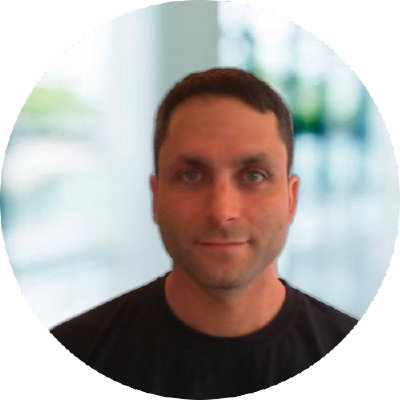
\includegraphics[width=0.4\textwidth]{images/santiago-lizardo.png}

	\begin{itemize}
		\item Reconmap's founder
		\item +20 years doing software engineering
		\item Cyber security enthusiast
		\item \href{https://github.com/santiagolizardo}{https://github.com/santiagolizardo}
	\end{itemize}
\end{frame}

\begin{frame}
	\frametitle{Reconmap's origin}

	Pentesting pain points	
	\begin{itemize}
		\item Repetition	
		\item Ineffective collaboration
		\item Ineffective communication
	\end{itemize}
\end{frame}

\begin{frame}
	\frametitle{Reconmap's mission}
	
	Reconmap's mission is to accelerate the time it takes to do vulnerability assessment and pentesting, through the use of templating, automation and machine learning. From weeks to days, or days to hours.
\end{frame}

\begin{frame}
	\frametitle{Reconmap's approach}
	
	\begin{itemize}
		\item Templates to avoid repetition
		\item Automation and ML to speed up the process
	\end{itemize}
	
	\begin{block}{Result:}
		Pentesters spending more time doing research, and less time doing repetitive, boring, tedious work such as parsing files manually or creating handcrafted pentest reports for their clients.	
	\end{block}
\end{frame}


\begin{frame}
	\frametitle{Reconmap's Today - September 2021}
	
	\begin{itemize}
		\item 1 year old
		\item Open source and SaaS
		\item Small but growing community
		\item Used in production by people around the world
	\end{itemize}
\end{frame}

\begin{frame}{}
	\frametitle{Recomap's feature set}
	
    \begin{itemize}
        \item Client, project, tasks management all in one.
        \item Reusable project and vulnerability templates
        \item Automatic pentest report generation (HTML, PDF, DOCX)
        \item Command line interface (CLI) and Rest API
        \item Integrated browser terminal
        \item Can scale to teams and projects of any size.
        \item Stats dashboard, user roles, documents, markdown, audit log, integrated search, tagging, data import/export, ...
    \end{itemize}
\end{frame}

\begin{frame}
	\frametitle{Who is it for?}
	
	Any InfoSec professional:
	\begin{itemize}
		\item Blue, Purple and Red teams
		\item Pentesters
		\item Bug bounty hunters
		\item Ethical hackers
		\item Security researchers
	\end{itemize}
	
	Individual or teams
\end{frame}

\begin{frame}
	\frametitle{Pentesting step by step with Reconmap}
	
	\begin{enumerate}
		\item Create client
		\item Create project from scratch or template
		\item Complete tasks in the project. Some might require running command automation.
		\item Try exploit the vulnerabilities found
		\item Generate report for client and share
	\end{enumerate}
\end{frame}

\begin{frame}
	\frametitle{Step 1: Setup client}
\begin{tikzpicture}
  \node (img1) {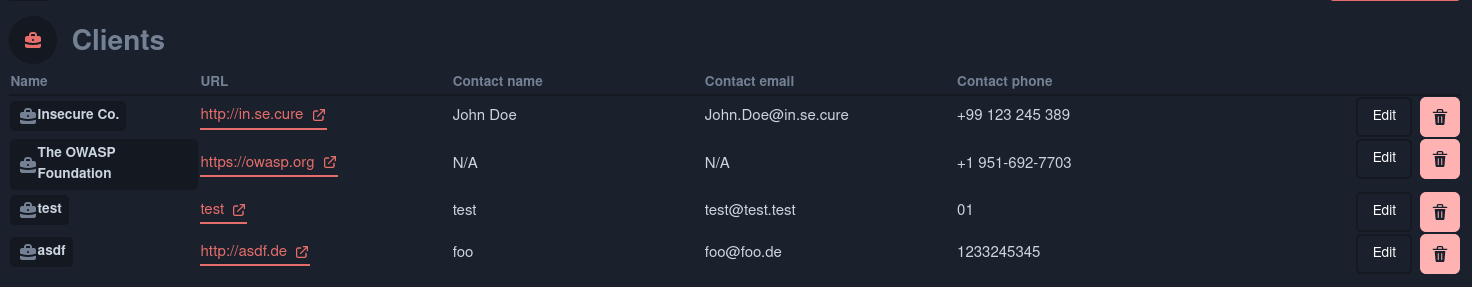
\includegraphics[height=2cm]{images/clients-list.png}};
  \pause
  \node (img2) at (img1.center) {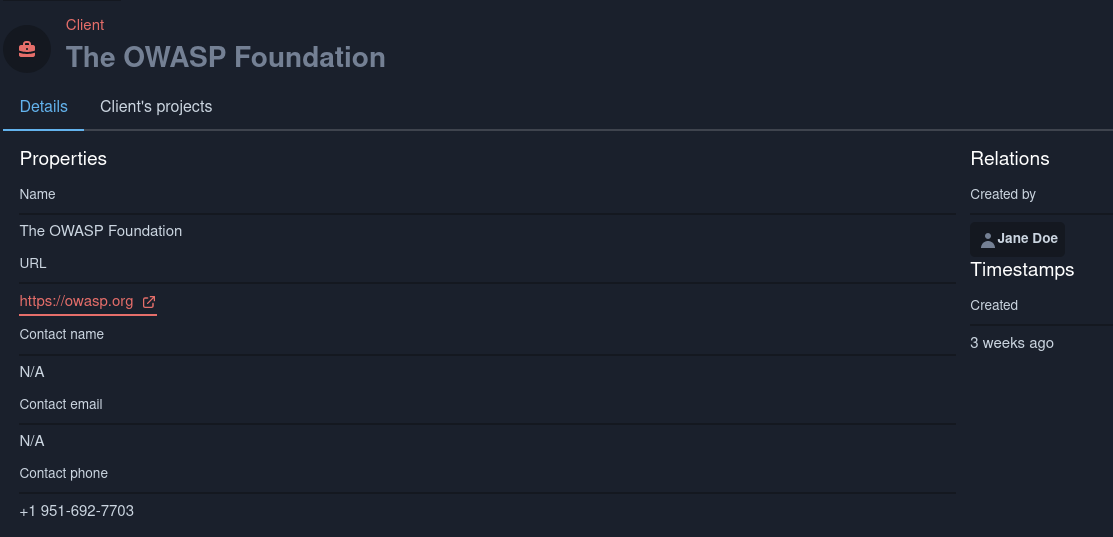
\includegraphics[height=3cm]{images/client-details.png}};
  \pause
  \node (img2) at (img1.south east) [xshift=-3cm] {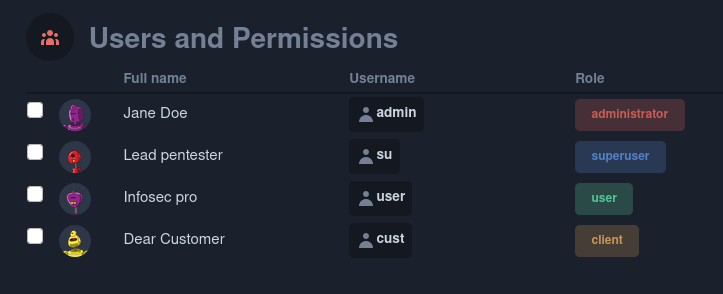
\includegraphics[height=3cm]{images/users-list.png}};
\end{tikzpicture}
\end{frame}

\begin{frame}
	\frametitle{Step 2: Setup project}
\begin{tikzpicture}
  \node (img1) {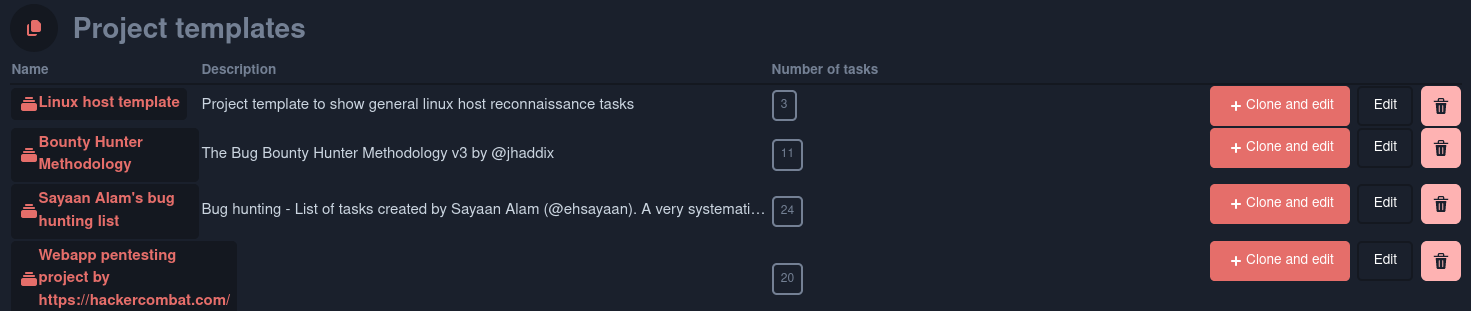
\includegraphics[height=2cm]{images/projects-list.png}};
  \pause
  \node (img2) at (img1.center) {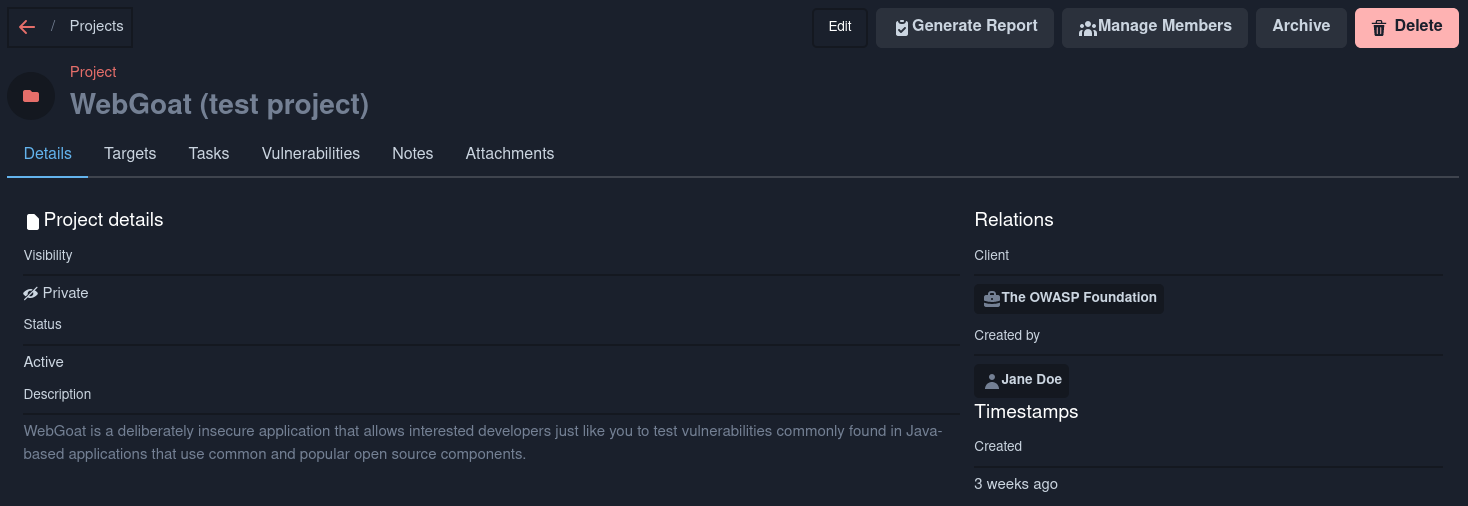
\includegraphics[height=3cm]{images/project-details.png}};
  \pause
  \node (img2) at (img1.south east) [xshift=-5cm] {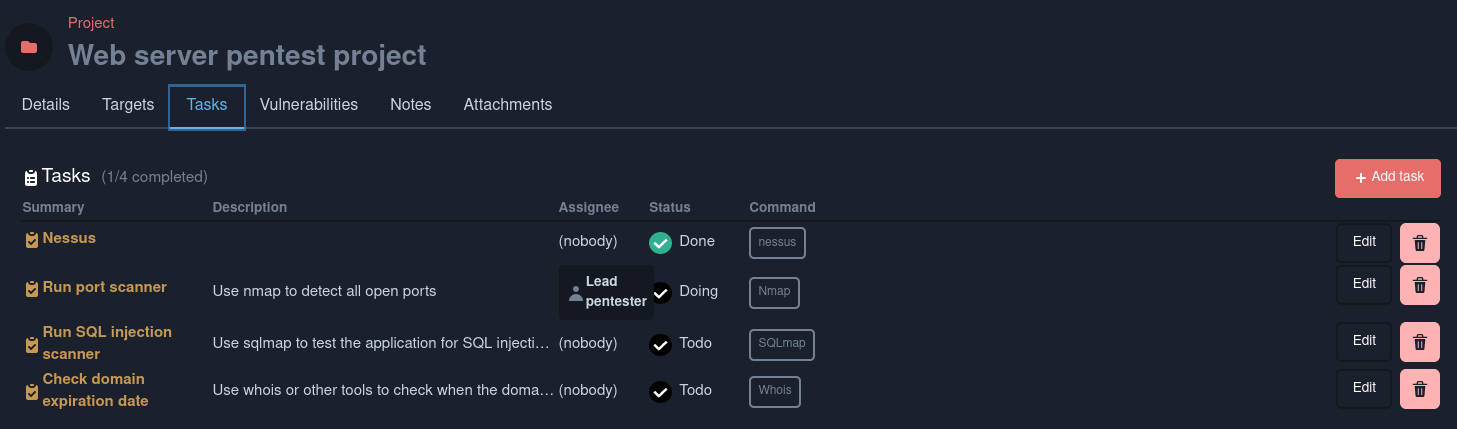
\includegraphics[height=3cm]{images/project-tasks.png}};
\end{tikzpicture}
\end{frame}

\begin{frame}
	\frametitle{Step 3: Complete tasks and commands}
\begin{tikzpicture}
  \node (img1) {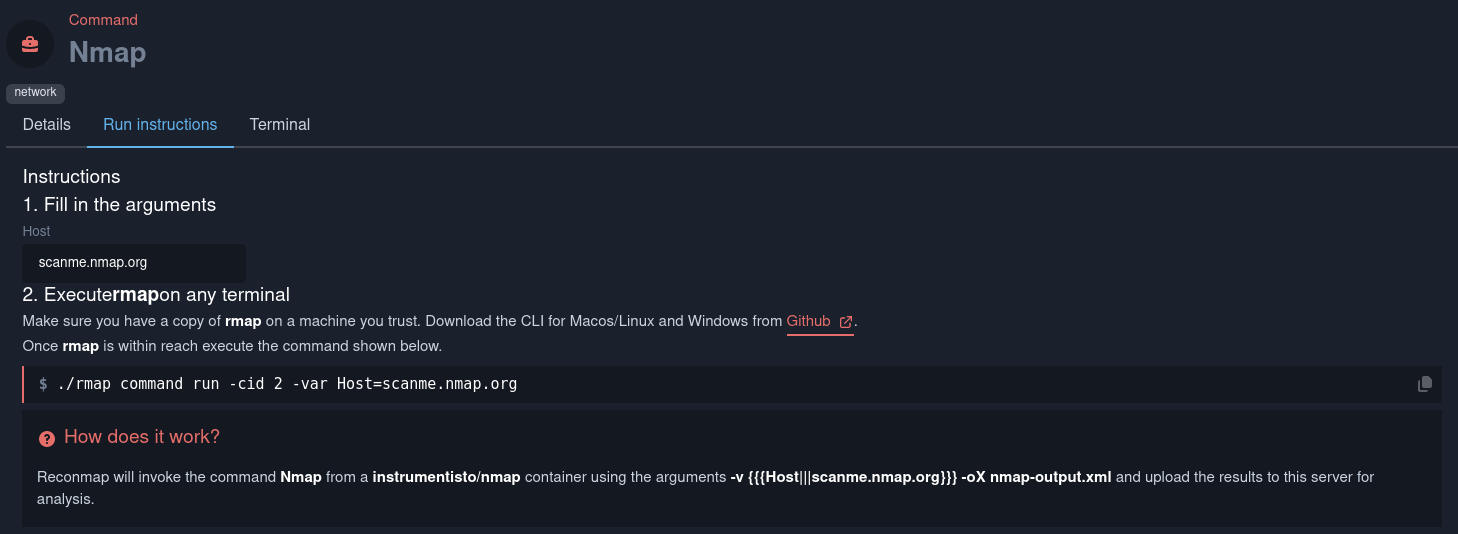
\includegraphics[width=0.8\textwidth]{images/command-run-instructions.png}};
  \pause
  \node (img2) at (img1.south east) [xshift=-5cm] {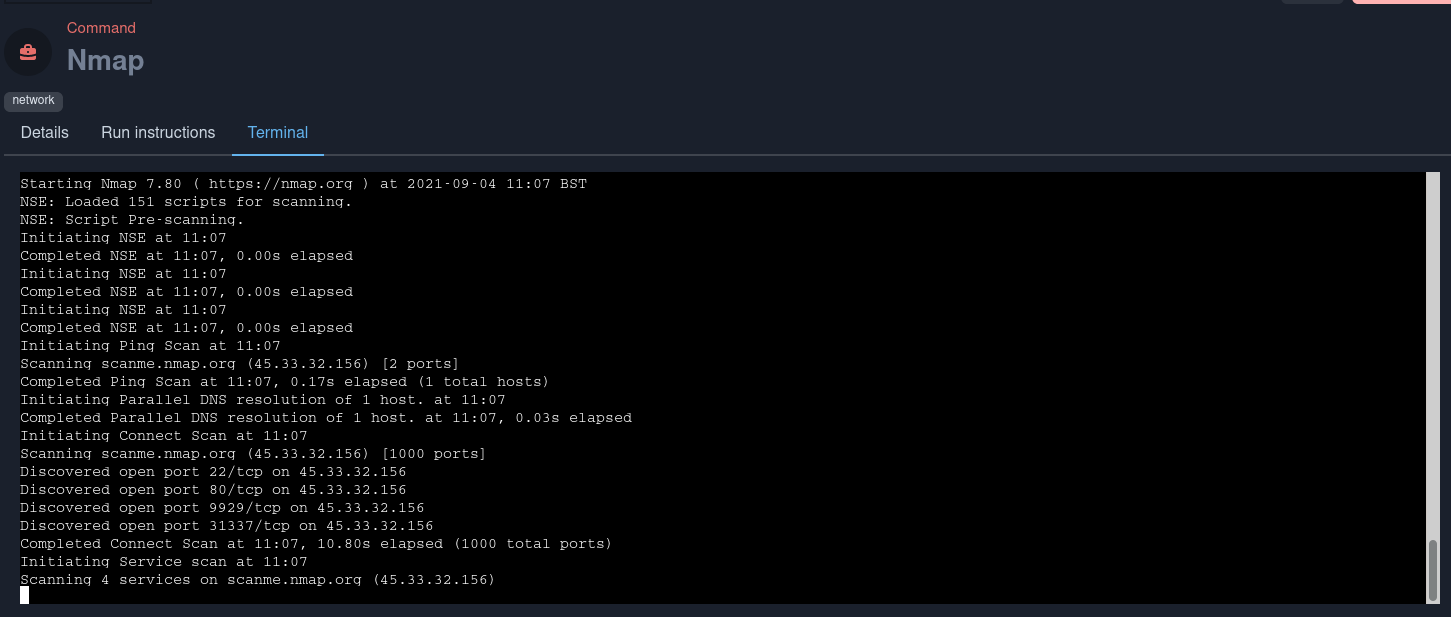
\includegraphics[height=4cm]{images/terminal-integration.png}};
\end{tikzpicture}
\end{frame}

\begin{frame}
	\frametitle{Step 4: Exploit vulnerabilities}
\begin{tikzpicture}
  \node (img1) {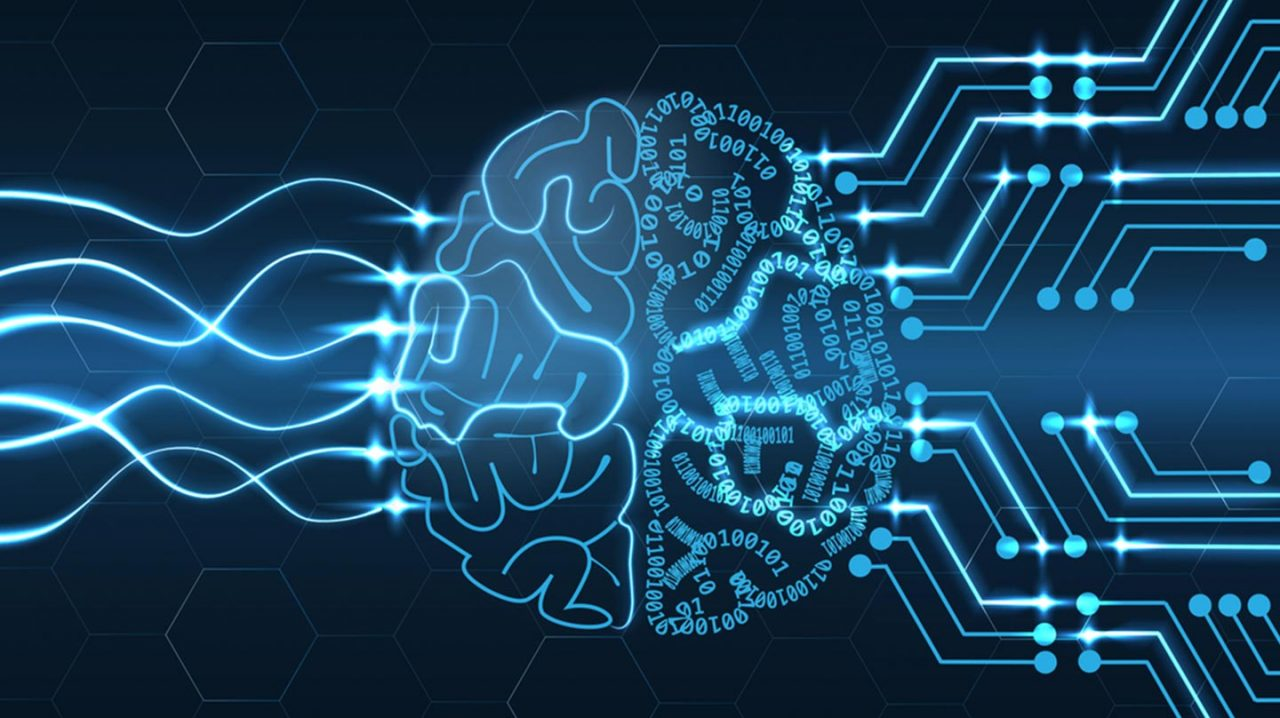
\includegraphics[height=3cm]{images/hacker-brain.jpg}};
  \pause
  \node (img2) at (img1.south west) {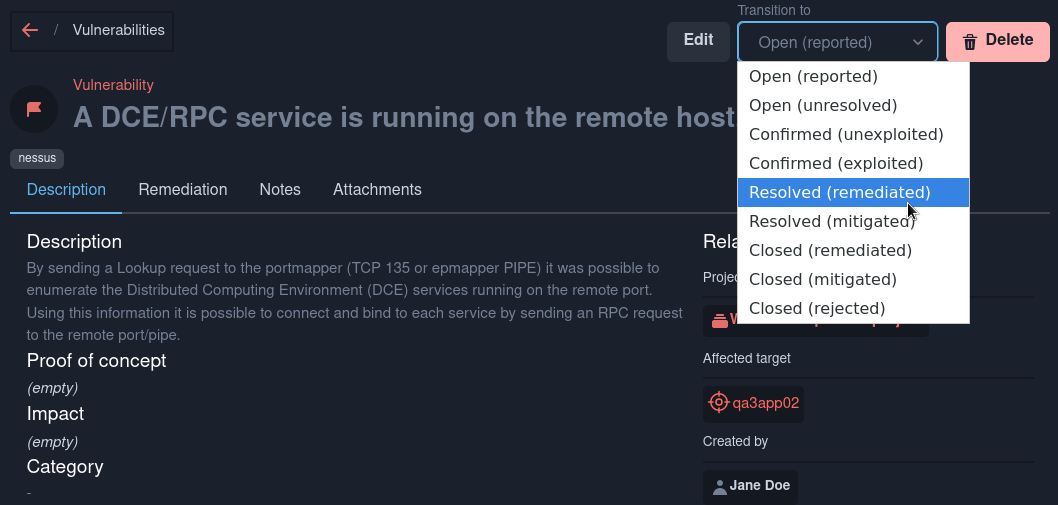
\includegraphics[height=5cm]{images/vulnerability-status.png}};
\end{tikzpicture}
\end{frame}

\begin{frame}
	\frametitle{Step 5: Generate pentest report}
\begin{tikzpicture}
  \node (img1) {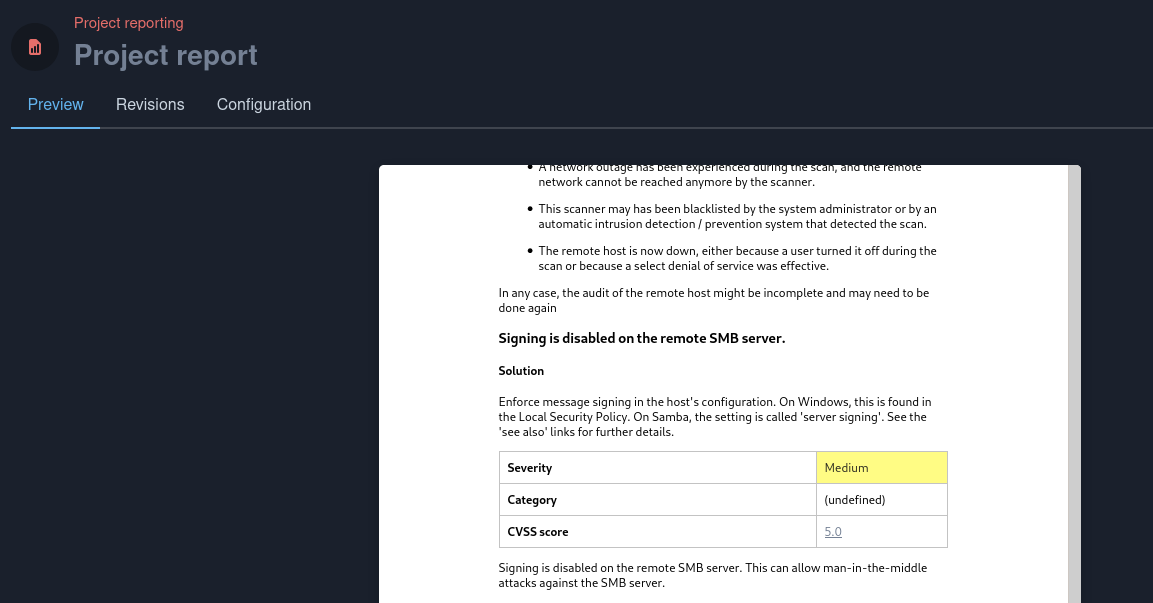
\includegraphics[height=3cm]{images/pentest-report-preview.png}};
  \pause
  \node (img2) at (img1.south east) {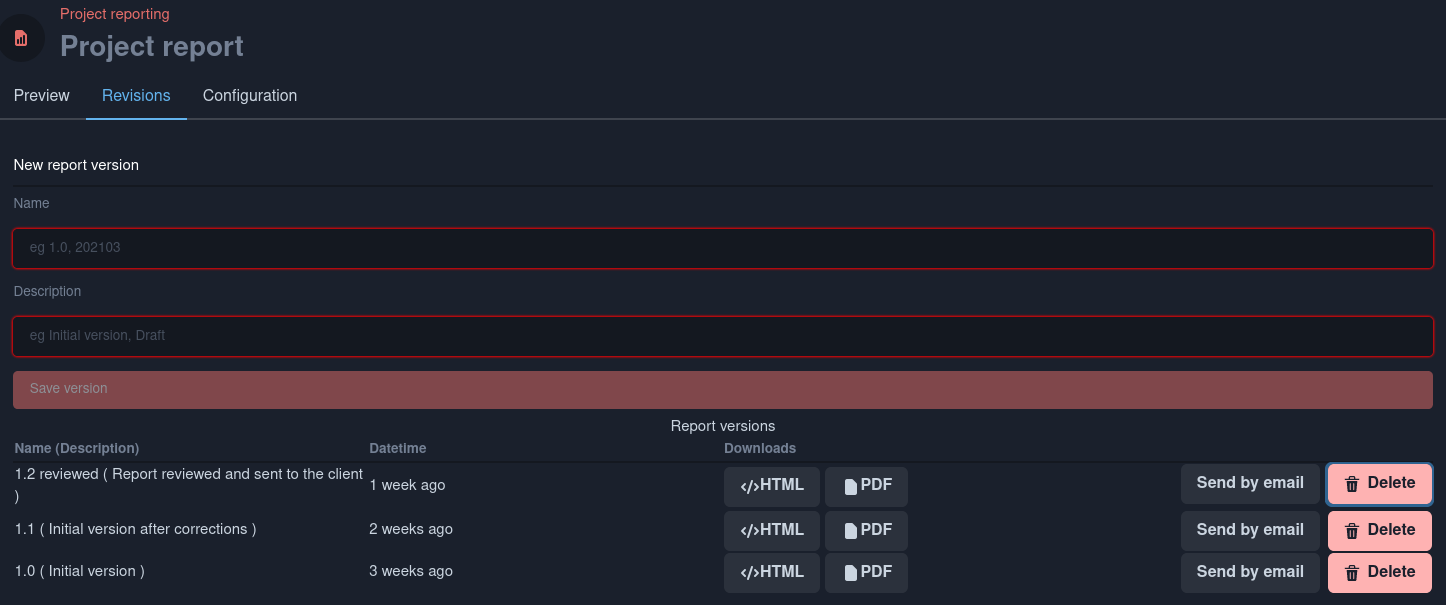
\includegraphics[height=3cm]{images/pentest-report-revisions.png}};
\end{tikzpicture}
\end{frame}

\begin{frame}
	\frametitle{Architecture}

	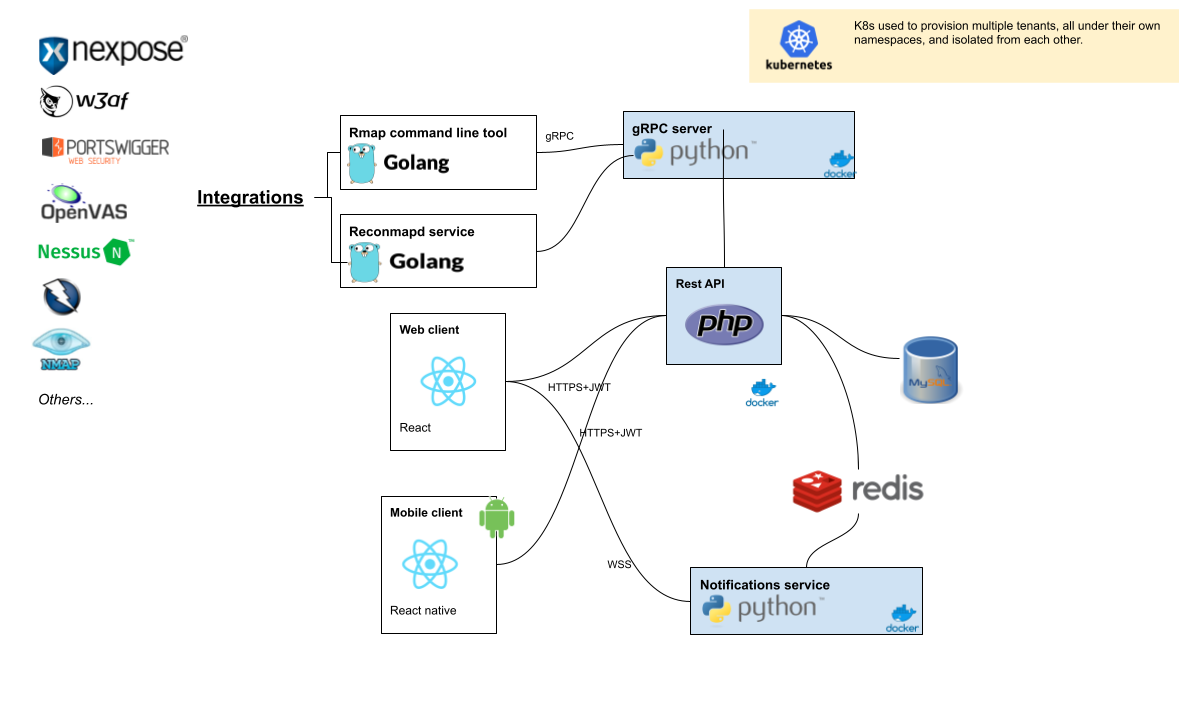
\includegraphics[width=\textwidth]{images/reconmap-architecture.png}
\end{frame}


\begin{frame}
	\frametitle{Coming features}
	
	\begin{itemize}
		\item Complex workflows (reviewers)
		\item Independent customer's portal
		\item Secret management
		\item More integrations
	\end{itemize}
\end{frame}

\section{How to get started?}

\begin{frame}{How to get started?}
    \begin{columns}[T]
        \begin{column}{.45\textwidth}
            \begin{block}{Manual setup}
            Follow \href{https://github.com/reconmap/reconmap\#readme}{setup instructions}\\
			\bigskip
            Requires significant time to install and maintain\\
            Community support (chat)
            \end{block}
        \end{column}
        \begin{column}{.45\textwidth}
            \begin{block}{SaaS}
            \href{https://reconmap.com}{Affordable hosting}\\
            \bigskip
            Ready in minutes\\
            Technical support (phone, email, chat)\\
            Always latest version            
            \end{block}
        \end{column}
    \end{columns}
    
\end{frame}

\section{Staying in touch}

\begin{frame}{Staying in touch}
	
\includegraphics[width=0.5\textwidth]{images/reconmap-logo.png}	
    \begin{itemize}
        \item \href{https://github.com/reconmap}{Github} community
        \item \href{https://twitter.com/reconmap}{Twitter} updates
        \item \href{https://facebook.com/reconmap}{Facebook}
        \item \href{https://gitter.im/reconmap/community}{Gitter} chat
    \end{itemize}
    \bigskip
	Pentester academy
    \begin{itemize}
        \item \href{https://twitter.com/DamianGoh13}{DamianGoh13}
        \item \href{https://www.pentesteracademy.com/}{Pentesteracademy.com}
    \end{itemize}
\end{frame}

\end{document}

